\chapter{Clustering Analysis (CA)}
\label{appendix_a}
\bibliographystyle{nar}
\section{General Methodology}
We considered  each of  the 20 non-A-RNA  type structures as  a vector
composed of  six base step  parameters.  We group these  vectors using
cluster analysis  following an automated process  shown to succesfully
reproduce well  known patterns of  the periodic table from  a selected
set  of variables, such  as, electronegativity,  ionization potential,
and  other elemental  properties  \cite{restrepo2004}.  The  procedure
followed  here  is  an  adaptation   of  how  clustering  is  used  to
re-construct the periodic table classification of the elements.

We start by normalizing the vectors of step parameters,
\begin{gather}
\label{eq:normalization}  
\overline{x}_{jA}=\frac{x_{jA}-x_{jmin}}{x_{jmax}-x_{jmin}}
\end{gather}
where ${x}_{jA}$ is the value  of the step parameter \textit{j} of the
structure A and $x_{jmin}$ and  $x_{jmax}$ are the minimum and maximum
values for a particular step parameter \textit{j} \cite{restrepo2006}.
Then,  using  the  software  package \textsf{R}  \cite{ihaka1996},  we
cluster these vectors into groups.  These groups can be displayed in a
tree  representation,  also called  a  dendrogram,  or  in biology,  a
phylogenetic tree (see Figure~\ref{fig:tree}).

To cluster  these vectors into groups,  it's necessary  to define the
distance between  the vectors. In  this work we used  three distance
definitions.   These distances  are  often referred  to as  Manhattan,
Euclidean  and   maximum  distances.  The  first   two  distances  are
particular cases of what is known as Minkowski's metric:
\begin{gather}
d(X,Y)= \Big( \sum_{i=1}^N |x_i-y_i|^k \Big)^\frac{1}{k}
\end{gather}
where $d(X,Y)$ refers to the distance between two vectors $X$ and $Y$,
where $N$ is  the dimensionality of the vector.  For  the case of step
parameters, $N$ is  six.  In the case where \textit{k}  is equal to 1,
the  definition  corresponds to  the  Manhattan  distance (a  distance
measured by  following along the edges  of blocks). In  the case where
\textit{k} is equal to 2, we have the familiar Euclidean distance. The
remaining distance, that is, the maximum distance, is defined by:
\begin{gather}
d(X,Y) = max |x_{i}-y_{i}|
\end{gather}
where  the  distance  between  vectors  $X$ and  $Y$  is  the  maximum
difference between vector variables.

\noindent Once the  distance si defined, we use  a hierarchical method
to cluster the space of distances between base-step parameters.
The clustering algorithm first finds the two closest vectors (given by
one of  the distance  definitions) and groups  them together.  Then it
compares the  distance of the elements  in the newly  formed group and
the  elements remaining  to be  grouped, according  to  the particular
clustering method.  For example,  the single linkage clustering method
takes  the  minimum  distance   between  elements  as  the  clustering
criterion.   Such  an  approach  would  (as  all  other  agglomerative
hierarchical methods do), group together the closest vectors given the
distance definition, and then would use the method definition (minimum
distance) to compare the distance of the elements of the group, to the
elements  which  remain  ungrouped,   or  to  the  elements  of  other
groups. As new  groups are formed the process  is repeated following a
hierarchical order,  that is, whatever  distance is smaller  gives the
grouping  criterion.   We   have  used  four  hierarchical  clustering
methods, the description of these methods follows in the next section,
"Hierarchical Methods".

For  every  possible combination  of  clustering  method and  distance
definition we  obtain a dendrogram. The combination  of three distance
definitions and four clustering  methods leads to 12 clustering trees.
These trees are not all exactly  the same but show recurring groups of
conformers.  To find the groups  which are repeated among the trees, a
consensus  analysis  is  performed  using  the  \textsf{clue}  package
\cite{hornik2005} implemented  in \textsf{R}. The  resulting consensus
tree is illustrated in Figure~\ref{fig:eucl_cons}.

\section{Hierarchical methods}
The hierarchical clustering methods used were:

\begin{enumerate}
\item{ \textit{Single linkage  clustering}, where the minimum distance
  between elements of each cluster is taken as clustering criteria.
\begin{gather}
D(X, Y)=min\{d(x_i, y_j): x_i \in X, y_j \in Y \}
\end{gather}
where  $X$ and  $Y$ are  vectors, and  $d(x_i, y_j)$  is  the distance
between cluster elements.  }

\item{  \textit{Complete   linkage  clustering},  where   the  maximum
  distance between cluster elements is the clustering criteria.
\begin{gather}
D(X, Y)=max\{d(x_i, y_j): x_i \in X, y_j \in Y \}
\end{gather} }

\item{ \textit{Average linkage  clustering}, the mean distance between
  elements of each cluster is taken as clustering criteria.
\begin{gather}
D(X, Y)=\frac{1}{N_x  * N_y} \sum_{i=1}^{N_x}  \sum_{j=1}^{N_y} d(x_i,
y_j)
\end{gather}
where  $N_x$  and $N_y$  are  the  number  of elements  in  respective
clusters.  }

\item{ \textit{Centroid linkage clustering}, uses the distance between
  cluster centroids, as clustering criteria.
\begin{gather}
D(X, Y)=d(\overline{x}, \overline{y})\\
\overline{x} = \frac{1}{N_x} \sum_{i=1}^{N_x} x_i\\
\overline{y} = \frac{1}{N_y} \sum_{i=1}^{N_y} y_i
\end{gather} }

\item{ \textit{Ward's  Method}, uses the  error sum of  squares (ESS).
%This Error Sum of Squares might  be the same as the residual sum of
%squares which is important in regression models.
\begin{gather}
D(X,Y)=ESS(XY) -[ESS(X) + ESS(Y)]\\
ESS(X)=  \sum_{i=1}^{N_x} \left|
x_i -\frac{1}{N_x}\sum_{j=1}^{N_x} x_j\right|^2
\end{gather} }
\end{enumerate}

As an example lets think of a case where we have five structures. Each
one of  them is descibed by  a bidimensional vector  as illustrated in
Table~\ref{tab:data}.
\begin{table}
\centering
\begin{tabular}[h]{|c|c|c|}
\hline
Structure & Property I & Property II\\
\hline\hline
1  &     1.00  &  5.00 \\
\hline
2  &    -2.00  & 6.00 \\
\hline
3  &      2.00  & -2.00 \\
\hline
4  &     -2.00  & -3.00 \\
\hline
5  &     3.00  &  -4.00 \\
\hline
\end{tabular}
\caption{Example of  structures, considered as  bidimensional vectors,
  to be clustered  using the average linkage method  and the Manhattan
  distance.}
\label{tab:data}
\end{table}

The  first step  is  to chose  a  distance definition.   We chose  the
Manhattan distance.  The  Manhattan distance values between structures
can be displayed in a  lower triangular matrix (usually refered simply
as the distance matrix) as seen in equation~\ref{eq:man}
\begin{gather} 
d(X, Y)=
\begin{vmatrix}
   & 1  &  2   & 3 & 4 & 5 \\
1  & 0  &      &   &   &   \\
2  & 4  &  0   &   &   &   \\
3  & 8  & 12   & 0 &   &   \\
4  & 11 &  9   & 5 & 0 &   \\
5  & 11 & 15   & 3 & 6 & 0 \\
\end{vmatrix}
\label{eq:man}
\end{gather}

Now,  let's  calculate  explicitily  the  Manhattan  distance  between
structures 2 and 3,

\begin{gather}
d(2, 3)= |-2.00 - 6.00| + |2.00 - -2.00| = 12
\end{gather}

Once we have calculated the  distances we pick a clustering method, in
this case,  we will use  the average linkage clustering  method. There
are two hierarchical techiques called agglomerative, or bottom-up, and
divisive, or  top-down. We will use the  agglomerative technique, that
is, going  from the bottom where  no objects are grouped,  to the top,
where all objects  constitute one final group. The  first step is then
to group whatever  structures are closer, that is,  structures 3 and 5
($d(3, 5)=3$). Now  we find the mean distance  between the elements of
this  cluster  and  the  remaining unclustered  structures,  that  is,
structures 1, 2 and 4, we obtain the following mean distances
\begin{gather}
D(\{3,5\}, 1)=\frac{1}{2*1}*(8+11) = 4.5 \label{eq:dist}\\
D(\{3,5\}, 2)=\frac{1}{2*1}*(12+15) = 13.5\\
D(\{3,5\}, 4)=\frac{1}{2*1}*(5+6) = 5.5
\end{gather}
Since  the distances between  \{3, 5\}  and all  remaining unclustered
vectors is  higher than  the distance between  vectors 1 and  2 ($d(1,
2)=4$) then \{1, 2\} are grouped. The following value, in hierarchical
increasing   order   is   4.5    between   \{3,   5\}   and   1   (see
equation~\ref{eq:dist}),  but since  1 and  2 are  already  grouped we
can't group  \{3, 5\} with 1.  The next value, following  the lower to
higher hierarchy,  is 5 ($d(3, 4)=5$),  but we have  already grouped 3
with 5, so we have to  keep advancing in the hierarchy. The next value
is 5.5, which  corresponds to grouping \{3, 5\} with  4, so we cluster
them. The only  remaining possibility for grouping is,  group \{1, 2\}
and \{4, 3, 5\}, so we do it as illustrated in Figure~\ref{fig:tree}.
\begin{figure}[t]
\centering
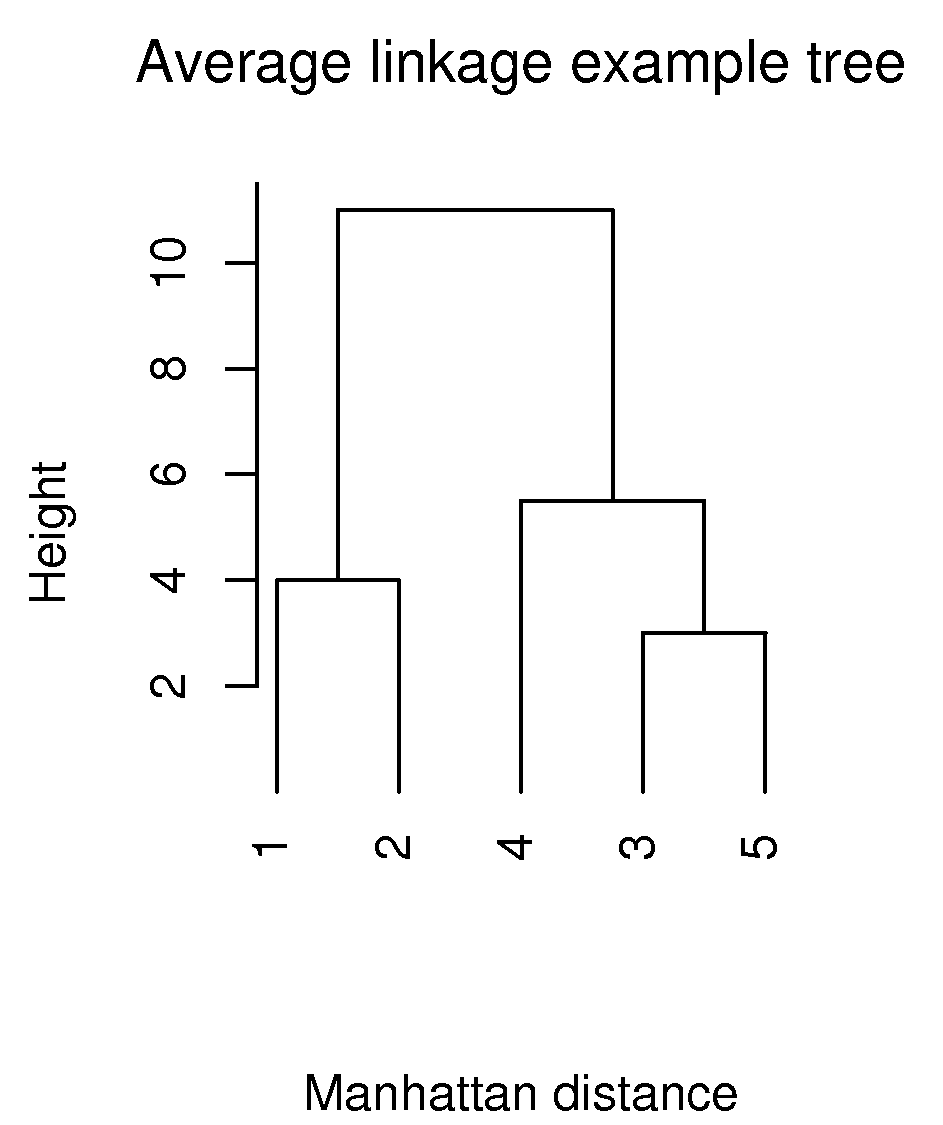
\includegraphics[scale=0.3]{Appendix/appendixtree.png}
\caption{Clustering  tree  for   5  bidimensional  vectors  using  the
  Manhattan  distance definition  and the  average  linkage clustering
  method.}
\label{fig:tree}
\end{figure}

\section{Clustering Validation Techniques}
The main objective of automated  clustering methods is that of finding
a reduced number of groups which share common characteristics in large
datasets. The main problem with the practical approaches used to solve
this task is that clustering methods do not offer 'a priori' an answer
to the  optimal number  of groups  that a large  dataset can  be split
into. In  our simple example  shown in Figure \ref{fig:tree}  our data
splits into two main groups.  Since this assesment is dependent on the
distances  and clustering methods  used in  particular cases,  then an
emergent necessity is that of  being able to determine the validity of
an   optimal  number   of  clusters   solution.   Such   methods,  not
surprisingly, are  known as clustering validation  techniques, and are
crucial  in the analysis  of the  gigantic amounts  of data  which are
being produced in the  the post-genomic boom of biological information
\cite{handl2005}, having  as a particular  case the one dealt  with in
this thesis.

We have  used the package clValid \cite{brock2008}  which implements a
variety  of  clustering validation  algorithms  using the  programming
language  \textbf{R}  \cite{rcite}.   The  clValid  package  comprises
measures which reflect  the compactness, connectedness, and separation
of cluster partitions. The concept  of compactness of a cluster refers
to the extent of  intra-cluster variation, the conectedness concept is
a more local  concept and means that neighboring  data elements should
belong to the same cluster, and the separation concept quantifies the
degree of separation between individual clusters. An illustration of
this concepts can be seen in Figure \ref{fig:concomsep}.

\begin{figure}
\centering
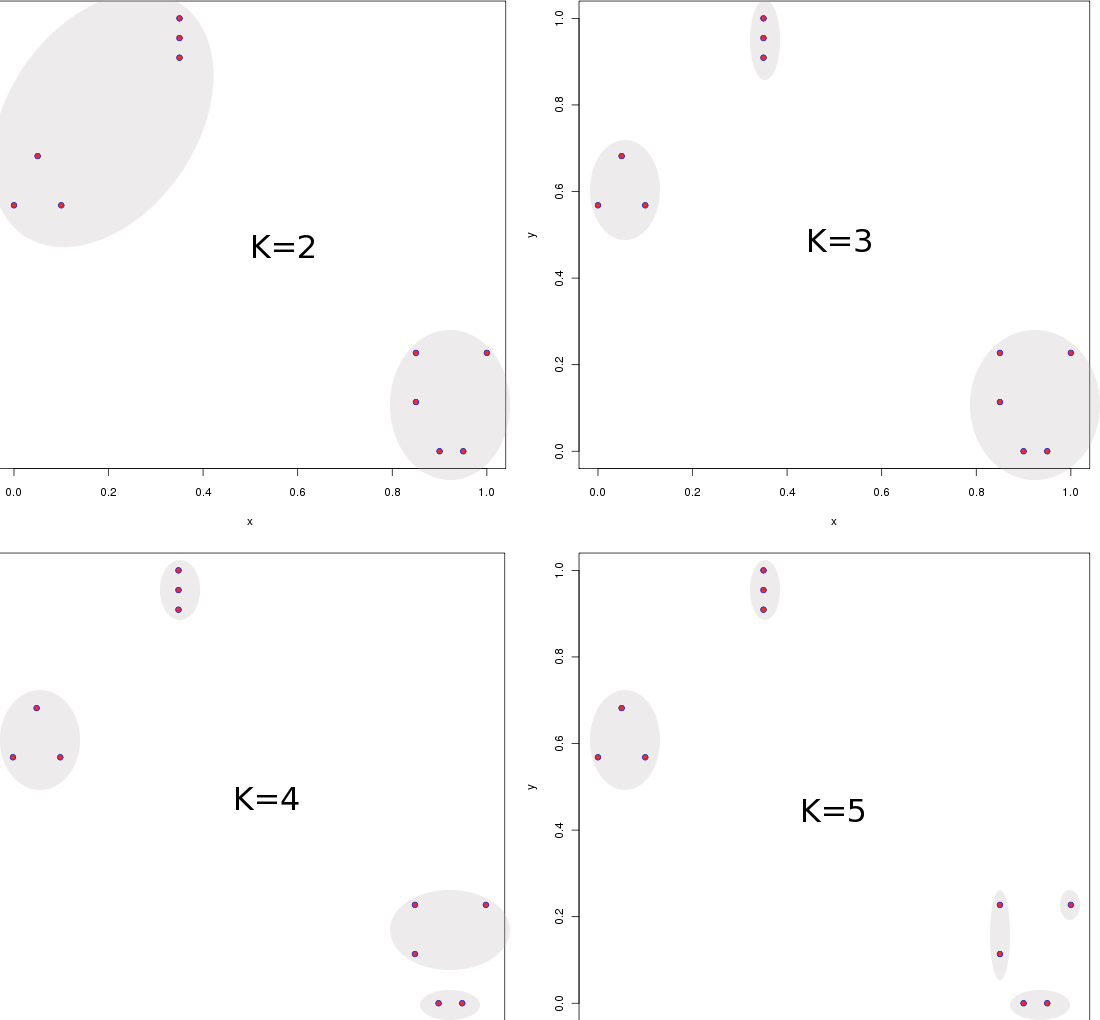
\includegraphics[scale=0.3]{Appendix/consilcom.png}
\caption{In this  figure we illustrate in a  bidimensional toy example
  the  concepts  of compactness,  connectedness,  and separation.   In
  images a)  trough d) we  have solutions for  hierarchical clustering
  considering $K=[2-5]$  clusters. For the  case of three  clusters we
  can  see that  compared to  the other  solutions, it  appears  to be
  composed of  more compact and  separated groups, this fact  would be
  quantified in  clValid with the asw  index and the  Dunn Index. For
  the two cluster  solution we see that it  is clearly more connected
  than  all other solutions,  but we  can also  appreciate that  as we
  group  data into  more clusters  connectivity will  be progressively
  lost just due to the fact of splitting data appart.}
\label{fig:concomsep}
\end{figure}  

\subsection{Internal Measures}
There are two main types of measures in the clValid package, these are
called internal measures, and stability measures. In general, internal
measures are those which use, exclusively, the dataset, the clustering
partitions,  and intrinsic  information in  the data  to  quantify the
quality of a  clustering result. In clValid three  indices are used to
account for compactness, conectedness and separation, the connectivity
index is used to measure cluster connectedness, and the the silhouette
width  and  Dunn index  combine  measures  of  cluster separation  and
compactness.

\subsubsection{Connectivity Index}
The connectivity index is defined as:
\begin{gather}
Conn(\mathcal{C}) = \sum_{i=1}^{N}\sum_{j=1}^{L} x_{i,nn_{i(j)}}
\end{gather}
Where $nn_{i(j)}$ stands for the $j^{th}$ nearest neighbor (nn) to the
$i^{th}$ observation.  If $i$,  and it's neareast neighbor $nn_{i(j)}$
are in  the same  cluster the term  $x_{i,nn_{i(j)}}$ is zero,  and if
they don't  belong to the  same cluster then  this term is  assigned a
value of $1/j$.  The parameter $L$ resembles a radius, in
the sense that it determines how many nearest neighbors are taken into
account per connectivity weight.
\begin{gather}
x_{i,nn_{i(j)}} =
    \begin{cases}
      0           &  \text{if } i \text{ and } nn_{i(j)} \in C_{k} \\
      \frac{1}{j} &  \text{otherwise.}
    \end{cases}
\end{gather}  
The  connectivity is  defined  for a  particular clustering  partition
$\mathcal{C} =  {C_{1},..., C_{K}}$, that is, for  a particular number
of clusters $K$ where the total number of observations is $N$. 
The connectivity index can give values between zero and $\infty$,
and smaller values mean better connectivity.

\subsubsection{Average Silhouette Width}
The average silhoutte width is the mean of silhoutte values $S(i)$
for $n$ observations.
\begin{gather}
asw = \frac{1}{n} \sum_{i=1}^{n} S(i)
\end{gather}  
The silhoutte value is defined as:
\begin{gather}
\label{eq:silval}  
S(i) = \frac{b_{i}-a_{i}}{\max(a_{i},b_{i})}
\end{gather}
Where $a_{i}$ is the average dissimilarity of observation $i$ to other
observations inside the cluster $i$ belongs to, and
$b_{i}$ is the average dissimilarity of observation $i$ to to
observations outside its own cluster. 
\begin{gather}
a_{i} = \frac{1}{n(C(i))} \sum_{j \in C(i)} d(i,j)\\
b_{i} = \min_{C_{k} \in \mathcal{C}} \sum_{j \in C_{k}}\frac{d(i,j)}{n(C_{k})}
\end{gather}  
The dissimilarity $d(i,j)$ is usually just a distance, for example the
Euclidean of  Manhattan distances, although formally it  does not need
to be  a metric, hence a  dissimilarity.  Notice that  due to equation
\ref{eq:silval}  the  average silhoutte  width  (asw)  can only  have
values    in   the    range   $[-1:1]$.     Kaufman    and   Rousseeuw
\cite{kaufman1990}  suggest  that  acceptable classifications  usually
have an asw value above 0.5  and those with values below 0.2 should be
considered as not  well classified.  Notice in the  lower left plot of
Figure   \ref{fig:internal}  that   all  values   for   validation  of
hierachical clustering for  single-base step-parameters are above 0.5.
The  asw  is  then  an  index  which  quantifies  the  separation  and
compactness of clustering solutions.

\subsubsection{Dunn Index}
The Dunn index is  similar to the asw index in the  sense that it also
quantifies the separation and  compactness of clustering solutions. It
is   an  index  which   measures  the   ratio  between   the  smallest
inter-cluster  distance and  the largest  intra-cluster distance  in a
partitioning.  The index is defined by:
\begin{gather}
D(C) = \min_{C_{k} \in C} \left(  \frac{\min_{C_{l} \in C}
  d(C_{k},C_{l})}{\max_{C_{m} \in C} diam(C_{m})} \right)
\end{gather}
Where $\min_{C_{l \in C}} d(C_{k},C_{l})$ is the minimum inter-cluster
distance,  and  $\max_{C_{m}  \in   C}  diam(C_{m})$  is  the  maximum
intra-cluster distance.   The Dunn index can have  values between zero
and $infty$, and a higher  value means a better cluster separation and
compactness.

\subsection{Stability Measures}
Stability  measures  are a  special  type  of  internal measure  which
evaluate  the   consistency  of  a  clustering   result  by  comparing
clusterings after sequential removal of a column of data.







%\newline
%Distance can be defined by Minkowski's metric:
%\begin{gather}
%d(X,Y)= \Big( \sum_{i=1}^N |x_i-y_i|^k \Big)^\frac{1}{k}
%\end{gather}
%In the particular case when $k=1$ we have the definition of the
%Manhattan or taxi-cab distance and when $k=2$ it's the familiar
%Euclidean distance.

%Finally, we can also define a maximum distance as the maximum
%difference between vectors variables.
%\begin{gather}
%d(X,Y) = max |x_{i}-y_{i}|
%\end{gather}

\bibliography{biblio}


